\documentclass[tikz,border=12pt]{standalone}
\usepackage[T1]{fontenc}
\usepackage{tgheros}
\usepackage{sfmath}
\usepackage{amsmath,amssymb}
% % \usepackage{fontawesome5} (Removed for publication-grade academic typography) (Removed for publication-grade academic typography)
\usepackage{tikz}
\usetikzlibrary{arrows.meta,positioning,shapes.geometric,fit,backgrounds,calc,decorations.pathreplacing}
\usepackage{xcolor}

\renewcommand{\familydefault}{\sfdefault}

% Academic Semantic Palette
\definecolor{ethdarkblue}{HTML}{1B2A4A}
\definecolor{ethslate}{HTML}{475569}
\definecolor{cardbg}{HTML}{F8FAFC}
\definecolor{cardborder}{HTML}{CBD5E1}
\definecolor{measuredTeal}{HTML}{168F84}
\definecolor{tealBg}{HTML}{E4F6F3}
\definecolor{proposalAmber}{HTML}{C98218}
\definecolor{amberBg}{HTML}{FFF3DC}
\definecolor{consequenceCoral}{HTML}{BD4F2F}
\definecolor{coralBg}{HTML}{FAE9E2}
\definecolor{authorityViolet}{HTML}{6550A8}
\definecolor{violetBg}{HTML}{F0ECFA}

\begin{document}
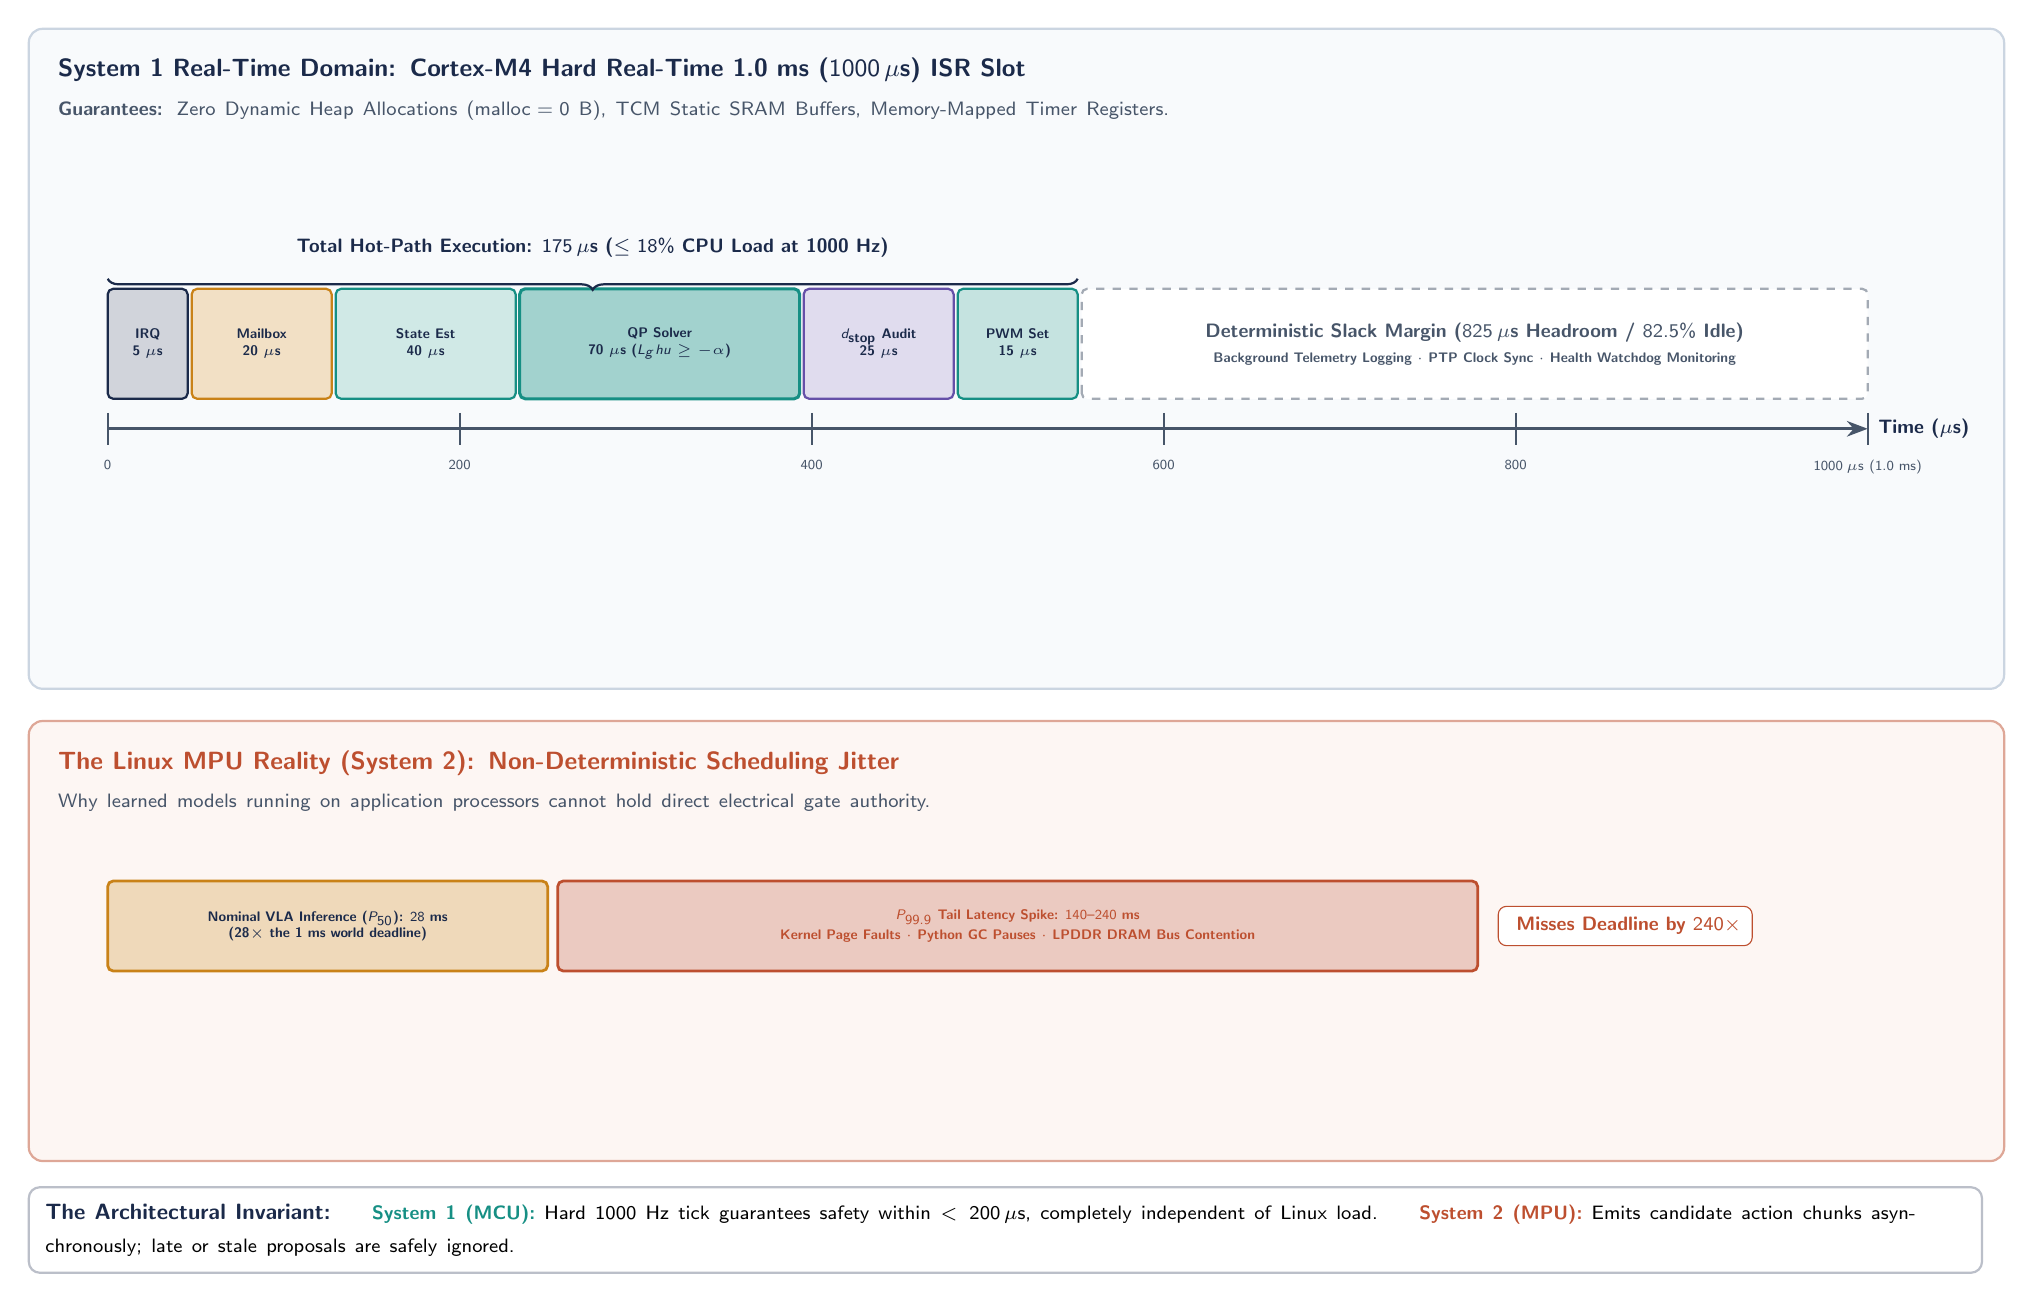
\begin{tikzpicture}[
  font=\sffamily,
  >=Stealth
]

  % Top Title Banner
  % (Top title banner removed for academic publication standards)
  % --- TOP CARD: The 1000 Hz / 1.0 ms Microcontroller Hard Loop ---
  \node[draw=cardborder, fill=cardbg, rounded corners=5pt, line width=0.8pt, text width=9.60in, minimum height=3.30in, inner sep=10pt, anchor=north west] (card_mcu) at (0,0) {};

  \node[anchor=north west, text width=9.30in, align=left, inner sep=0pt] at ($(card_mcu.north west)+(0.15in,-0.15in)$) {
    {\small\bfseries\color{ethdarkblue} System 1 Real-Time Domain: Cortex-M4 Hard Real-Time 1.0 ms ($1000\,\mu\text{s}$) ISR Slot}\\[2pt]
    {\scriptsize\color{ethslate}\textbf{Guarantees:} Zero Dynamic Heap Allocations ($\text{malloc} = 0\text{ B}$), TCM Static SRAM Buffers, Memory-Mapped Timer Registers.}
  };

  % Timing Waterfall Bars (Total width = 8.80 inches representing 1000 us)
  \coordinate (Worigin) at ($(card_mcu.west)+(0.40in, -0.35in)$);

  % Timeline Axis
  \draw[->, line width=1pt, ethslate] (Worigin) -- ++(8.80in, 0)
    node[right, font=\sffamily\bfseries\scriptsize, text=ethdarkblue] {Time ($\mu\text{s}$)};

  % Time tick marks
  \foreach \x/\label in {0/{0}, 1.76/{200}, 3.52/{400}, 5.28/{600}, 7.04/{800}, 8.80/{1000\,\mu\text{s}\;(1.0\text{ ms})}} {
    \draw[line width=0.6pt, ethslate] ($(Worigin)+(\x in, 0.08in)$) -- ($(Worigin)+(\x in, -0.08in)$)
      node[below=2pt, font=\sffamily\tiny, text=ethslate] {$\label$};
  }

  % Stage 1: Timer IRQ & Context Save (5 us -> visually 0.40 in)
  \draw[fill=ethdarkblue!20, draw=ethdarkblue, line width=0.8pt, rounded corners=2pt]
    ($(Worigin)+(0, 0.15in)$) rectangle ++(0.40in, 0.55in)
    node[midway, font=\sffamily\bfseries\tiny, text=ethdarkblue, align=center] {IRQ\\{\tiny 5 $\mu$s}};

  % Stage 2: IPC Mailbox Ingest (20 us -> visually 0.70 in)
  \draw[fill=proposalAmber!25, draw=proposalAmber, line width=0.8pt, rounded corners=2pt]
    ($(Worigin)+(0.42in, 0.15in)$) rectangle ++(0.70in, 0.55in)
    node[midway, font=\sffamily\bfseries\tiny, text=ethdarkblue, align=center] {Mailbox\\{\tiny 20 $\mu$s}};

  % Stage 3: State Est & FK (40 us -> visually 0.90 in)
  \draw[fill=measuredTeal!20, draw=measuredTeal, line width=0.8pt, rounded corners=2pt]
    ($(Worigin)+(1.14in, 0.15in)$) rectangle ++(0.90in, 0.55in)
    node[midway, font=\sffamily\bfseries\tiny, text=ethdarkblue, align=center] {State Est\\{\tiny 40 $\mu$s}};

  % Stage 4: KKT QP Barrier Solver (70 us -> visually 1.40 in)
  \draw[fill=measuredTeal!40, draw=measuredTeal, line width=1.1pt, rounded corners=2pt]
    ($(Worigin)+(2.06in, 0.15in)$) rectangle ++(1.40in, 0.55in)
    node[midway, font=\sffamily\bfseries\tiny, text=ethdarkblue, align=center] { QP Solver\\{\tiny 70 $\mu$s ($L_g h u \ge -\alpha$)}};

  % Stage 5: Dynamic Stopping Audit (25 us -> visually 0.75 in)
  \draw[fill=authorityViolet!20, draw=authorityViolet, line width=0.8pt, rounded corners=2pt]
    ($(Worigin)+(3.48in, 0.15in)$) rectangle ++(0.75in, 0.55in)
    node[midway, font=\sffamily\bfseries\tiny, text=ethdarkblue, align=center] {$d_{\text{stop}}$ Audit\\{\tiny 25 $\mu$s}};

  % Stage 6: PWM Timer Register Write (15 us -> visually 0.60 in)
  \draw[fill=measuredTeal!25, draw=measuredTeal, line width=0.8pt, rounded corners=2pt]
    ($(Worigin)+(4.25in, 0.15in)$) rectangle ++(0.60in, 0.55in)
    node[midway, font=\sffamily\bfseries\tiny, text=ethdarkblue, align=center] {PWM Set\\{\tiny 15 $\mu$s}};

  % Slack Headroom (Remaining 825 us -> visually 3.90 in)
  \draw[fill=white, draw=ethslate!50, dashed, line width=0.8pt, rounded corners=2pt]
    ($(Worigin)+(4.87in, 0.15in)$) rectangle ++(3.93in, 0.55in)
    node[midway, font=\sffamily\bfseries\scriptsize, text=ethslate, align=center] {
       Deterministic Slack Margin ($825\,\mu\text{s}$ Headroom / $82.5\%$ Idle)\\[1pt]
      {\tiny Background Telemetry Logging $\cdot$ PTP Clock Sync $\cdot$ Health Watchdog Monitoring}
    };

  % Total Hot-Path Callout Bracket
  \draw[thick, ethdarkblue, decorate, decoration={brace, amplitude=4pt}]
    ($(Worigin)+(4.85in, 0.75in)$) -- ($(Worigin)+(0, 0.75in)$)
    node[midway, above=4pt, font=\sffamily\bfseries\scriptsize, text=ethdarkblue] {
      \textbf{Total Hot-Path Execution: $175\,\mu\text{s}$ ($\le 18\%$ CPU Load at 1000 Hz)}
    };

  % --- BOTTOM CARD: Linux MPU Latency Tail Jitter ---
  \node[draw=consequenceCoral!50, fill=coralBg!40, rounded corners=5pt, line width=0.8pt, text width=9.60in, minimum height=2.20in, inner sep=10pt, below=0.15in of card_mcu.south west, anchor=north west] (card_mpu) {};

  \node[anchor=north west, text width=9.30in, align=left, inner sep=0pt] at ($(card_mpu.north west)+(0.15in,-0.15in)$) {
    {\small\bfseries\color{consequenceCoral} The Linux MPU Reality (System 2): Non-Deterministic Scheduling Jitter}\\[2pt]
    {\scriptsize\color{ethslate}Why learned models running on application processors cannot hold direct electrical gate authority.}
  };

  % Jitter comparison bar
  \coordinate (Morigin) at ($(card_mpu.west)+(0.40in, -0.20in)$);

  % Nominal MPU Latency
  \draw[fill=proposalAmber!30, draw=proposalAmber, line width=1pt, rounded corners=2pt]
    ($(Morigin)+(0, 0.05in)$) rectangle ++(2.20in, 0.45in)
    node[midway, font=\sffamily\bfseries\tiny, text=ethdarkblue, align=center] {
      \textbf{Nominal VLA Inference ($P_{50}$): $28\text{ ms}$}\\{\tiny (28$\times$ the 1 ms world deadline)}
    };

  % P99 Tail Blowout
  \draw[fill=consequenceCoral!30, draw=consequenceCoral, line width=1pt, rounded corners=2pt]
    ($(Morigin)+(2.25in, 0.05in)$) rectangle ++(4.60in, 0.45in)
    node[midway, font=\sffamily\bfseries\tiny, text=consequenceCoral, align=center] {
       \textbf{$P_{99.9}$ Tail Latency Spike: $140\text{--}240\text{ ms}$}\\[1pt]
      {\tiny Kernel Page Faults $\cdot$ Python GC Pauses $\cdot$ LPDDR DRAM Bus Contention}
    };

  % Consequence Callout Badge
  \node[draw=consequenceCoral, fill=white, rounded corners=3pt, font=\sffamily\scriptsize, text=consequenceCoral, inner sep=4pt, anchor=west]
    at ($(Morigin)+(6.95in, 0.275in)$) {
      \textbf{ Misses Deadline by $240\times$}
    };

  % Bottom Summary Strip
  \node[draw=ethdarkblue!30, fill=white, rounded corners=4pt, line width=0.8pt, text width=9.60in, inner sep=6pt, below=0.12in of card_mpu.south west, anchor=north west] (strip_btm) {
    {\footnotesize\textbf{\color{ethdarkblue}The Architectural Invariant:}} \quad
    {\scriptsize\textbf{\color{measuredTeal}System 1 (MCU):}} {\scriptsize Hard $1000\text{ Hz}$ tick guarantees safety within $<200\,\mu\text{s}$, completely independent of Linux load.} \quad
    {\scriptsize\textbf{\color{consequenceCoral}System 2 (MPU):}} {\scriptsize Emits candidate action chunks asynchronously; late or stale proposals are safely ignored.}
  };

\end{tikzpicture}
\end{document}
